\documentclass{standalone}
\usepackage{tikz}
\usepackage{ctex,siunitx,ninecolors}
\setCJKmainfont{Noto Serif CJK SC}
\usepackage{tkz-euclide}
\usepackage{amsmath}
\usetikzlibrary{patterns, calc}
\usetikzlibrary {decorations.pathmorphing, decorations.pathreplacing, decorations.shapes}
\newcommand\dynamometer[3][0]{
  \begin{scope}[#2,rotate=#1,inner sep=0pt]
    \coordinate (A) at (0,2.0);
    \coordinate (B) at (0,2.0+#3*0.2);
    \foreach \x/\y in {100/2.0, 70/1.5, 50/1.2, 30/0.7 }
    {
      \draw[line width=\y pt,gray!\x ]([yshift=1cm]B)circle(0.2);
    }
    \fill[top color=gray, bottom color=gray,middle color=white]([xshift=-1mm,yshift=7mm]B)rectangle([xshift=1mm,yshift=8.7mm]B);
    \fill[green!30!black]([xshift=2.8mm,yshift=6mm]B)--([xshift=2.8mm,yshift=-1.2cm]B)to[bend left=50]([xshift=-2.8mm,yshift=-1.2cm]B)--([xshift=-2.8mm,yshift=6mm]B)to[bend left=50]cycle;
    \fill[lightgray,even odd rule](0.1,0.4)arc(360:180:0.1)--++(0,1.6)--++(0.2,0)--cycle(0,0.4)circle(0.05)([xshift=-0.4mm]A)rectangle++(0.8mm,0.5mm);
    \fill[lightgray!30,even odd rule]([xshift=2.2mm,yshift=5mm]B)--([xshift=2.2mm,yshift=-1.1cm]B)to[bend left]([xshift=-2.2mm,yshift=-1.1cm]B)[rounded corners=2pt]--([xshift=-2.2mm,yshift=5mm]B)[sharp corners]--([xshift=-1mm,yshift=5mm]B)arc(180:0:0.1)[rounded corners=2pt]--cycle[sharp corners]
    ([xshift=-0.4mm,yshift=2mm]B)rectangle([xshift=0.4mm]A);
    \draw[darkgray](0.1,0.1)arc(360:90:0.1)--++(0,0.15);
    \foreach \x in {0,1,...,9}
    {
      \draw[line width=0.1pt,line join=round,lightgray]([yshift=2mm-\x*0.15mm-\x*#3*0.2mm]B)--++(0.3mm,-0.0375mm-#3*0.05mm)--++(-0.6mm,-0.075mm-#3*0.1mm)--++(0.3mm,-0.0375mm-#3*0.05mm);
    }
    \fill[red]([yshift=-0.2mm]A)--([xshift=-1mm]A)--([xshift=1mm]A);
    \foreach \x in {0,1,2,3,4}
    {
      \draw[ultra thin]([xshift=0.5mm,yshift=-\x*2mm]B)--++(0.07,0)node[rotate=#1,right]{\resizebox{!}{0.5mm}{\x}};
      \draw[ultra thin]([xshift=-0.5mm,yshift=-\x*2mm]B)--++(-0.07,0)node[rotate=#1,left]{\resizebox{!}{0.5mm}{\x}};
      \foreach \y in {1,2,3,4,6,7,8,9}
      {
        \draw[ultra thin]([xshift=0.5mm,yshift=-\x*2mm-\y*0.2mm]B)--++(0.05,0);
        \draw[ultra thin]([xshift=-0.5mm,yshift=-\x*2mm-\y*0.2mm]B)--++(-0.05,0);
      }
      \draw[ultra thin]([xshift=0.5mm,yshift=-\x*2mm-1mm]B)--++(0.06,0);
      \draw[ultra thin]([xshift=-0.5mm,yshift=-\x*2mm-1mm]B)--++(-0.06,0);
    }
    \draw[ultra thin]([xshift=0.5mm,yshift=-1cm]B)--++(0.07,0)node[rotate=#1,right]{\resizebox{!}{0.5mm}{5}};
    \draw[ultra thin]([xshift=-0.5mm,yshift=-1cm]B)--++(-0.07,0)node[rotate=#1,left]{\resizebox{!}{0.5mm}{5}};
  \end{scope}
  }
\begin{document}
\small
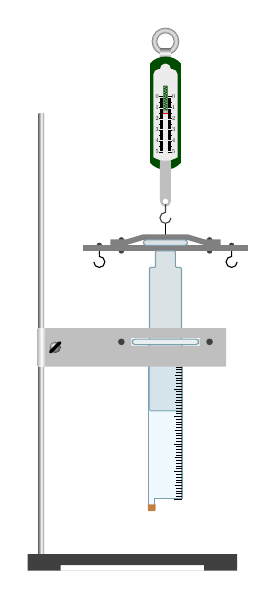
\begin{tikzpicture}[>=latex,scale=0.7]
  % \useasboundingbox(-1.4,-1.4)rectangle(1.4,1.4);
  \begin{scope}[xshift=-3mm,yshift=1.6cm]
    \fill[darkgray](-0.8,3.1)circle(0.05)(0.8,3.1)circle(0.05)(-0.8,2.9)circle(0.05)(0.8,2.9)circle(0.05)(1.2,3.0)circle(0.05)(-1.2,3.0)circle(0.05);
    \draw(0,3.1)--++(0,0.3);
    \draw(1.2,3)--++(0,-0.2)arc(90:360:0.1);
    \coordinate (A1) at (1.2,2.6);
    \draw(-1.2,3)--++(0,-0.2)arc(90:-180:0.1);
    \coordinate (B1) at (-1.2,2.6);
    \draw[very thick](-0.8,3.1)--(-0.8,2.9)(0.8,3.1)--(0.8,2.9);
    \fill[gray](-1.5,2.9)rectangle(1.5,3.0);
    \draw[gray,line width=0.7mm](-1.0,3.06)--(-0.7,3.06)--(-0.4,3.15)--(0.4,3.15)--(0.7,3.06)--(1.0,3.06);
    \draw[cyan!30!gray,fill=cyan!10!lightgray!50,rounded corners=0.14mm](-0.29,0)--(-0.29,2.6)--(-0.18,2.6)--(-0.18,2.9)--(0.18,2.9)--(0.18,2.6)--(0.29,2.6)--(0.29,0)--cycle;
    
    \draw[cyan!30!gray,fill=cyan!10!lightgray!50,rounded corners=0.35mm](-0.4,3.0)rectangle(0.4,3.1);
  \end{scope}
  \draw[cyan!30!gray,fill=cyan!20,fill opacity=0.3](0,0)--(-0.5,0)--(-0.5,-0.2)--(-0.6,-0.2)--(-0.6,2.8)--(0,2.8)--cycle;
  \draw[cyan!30!gray,fill=cyan!10!lightgray!30,rounded corners=0.35mm](-0.9,2.8)rectangle(0.3,2.9);
  \fill[brown,rounded corners=0.14mm](-0.62,-0.1)--(-0.62,-0.22)--(-0.48,-0.22)--(-0.48,-0.1);
  \foreach \y in {0,0.5,...,2.0}
  {
    \draw[ultra thin](0,\y)--++(-0.15,0);
    \draw[ultra thin](0,\y+0.25)--++(-0.12,0);
    \foreach \z in {1,2,3,4,6,7,8,9}
    {
      \draw[ultra thin](0,\y+0.05*\z)--++(-0.10,0);
    }
  }
  \draw[ultra thin](0,2.5)--++(-0.15,0);
  \fill[lightgray,even odd rule](-2.48,2.4)rectangle(0.8,3.1)(-0.92,2.78)rectangle(0.32,2.92);
  \fill[darkgray](-1.1,2.85)circle(0.06)(0.5,2.85)circle(0.06);
  \fill[left color=gray,right color=gray,middle color=white](-2.5,-1.0)rectangle(-2.6,7.0);
  \fill[left color=lightgray,right color=lightgray,middle color=white](-2.48,2.4)rectangle(-2.62,3.1);
  \fill[ball color=lightgray](-2.3,2.75)circle(0.1);
  \draw[very thick,line cap=round]([shift=(-135:0.12)]-2.3,2.75)--++(45:0.24);
  \fill[darkgray,even odd rule](-2.8,-1.0)rectangle(1.0,-1.3)(-2.2,-1.2)rectangle(0.4,-1.3);
  % \fill[left color=gray,right color=gray,middle color=white]([xshift=-2mm]B1)rectangle++(0.4,-0.5);
  % \fill[left color=gray,right color=gray,middle color=white]([xshift=-2mm]A1)rectangle++(0.4,-0.5);
  \dynamometer{xshift=-3mm,yshift=5cm}{1.5}
\end{tikzpicture}
\end{document}